%source mathadata
\begin{multicols}{2}
		Un algorithme cherche la meilleure droite de séparation entre les ronds et les carrés. Pour cela, il modifie pas à pas l'ordonnée à l'origine $p$ tout en gardant le coefficient directeur $m$ fixe.

		\begin{itemize}
			\item La droite de séparation $D_1$ tracée sur le graphique est un premier essai.
			\item Au-dessus de la droite, c'est la zone des ronds et en dessous celle des carrés.
		\end{itemize}

	\end{multicols}

	\begin{center}
		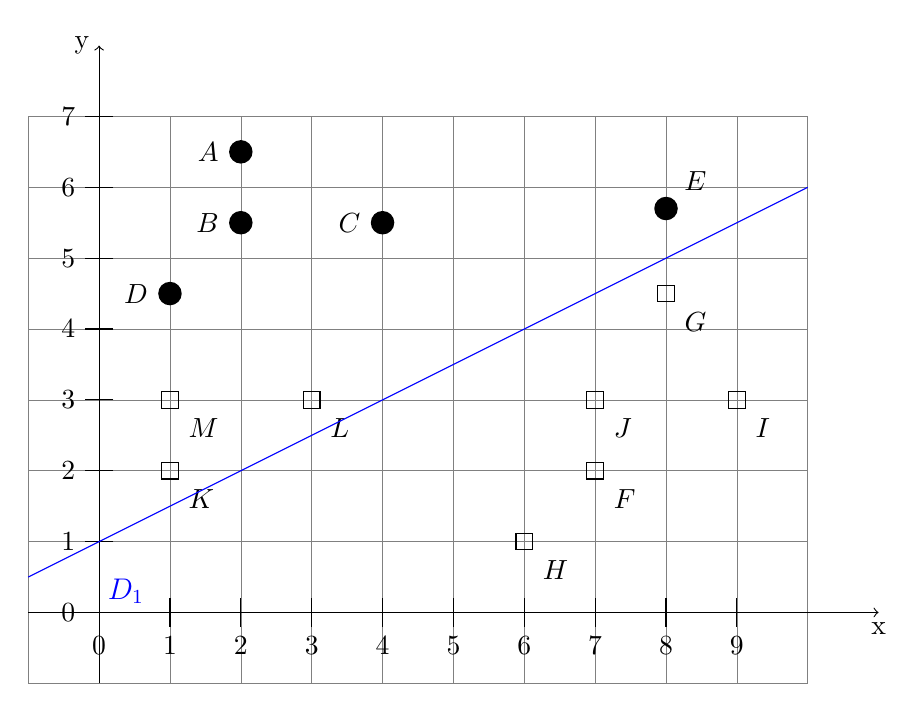
\begin{tikzpicture}[scale=0.9]
			% \tikzstyle{subj} = [circle, minimum width=4pt, fill, inner sep=0pt]
			% \tikzstyle{obj}  = [circle, minimum width=8pt, draw, inner sep=0pt]

			\tikzset{
				grid major/.style = {very thin, gray},
				grid minor/.style = {very thin, lightgray}
			}
			\draw[grid major] (-1, -1) grid[step=1] (10, 7);
			\draw[->] (-1,0) -- (11,0) node[below] {x};
			\draw[->] (0,-1) -- (0,8) node[left] {y};
			\foreach \x in {0,1,...,9} \draw (\x,0.2) -- (\x,-0.2) node[below] {\x};
			\foreach \y in {0,1,...,7} \draw (0.2,\y) -- (-0.2,\y) node[left] {\y};
			\node at (2,6.5) [circle,fill,inner sep=3pt,label=left:{$A$}] {}; % Mouton A
			\node at (2,5.5) [circle,fill,inner sep=3pt,label=left:{$B$}] {}; % Mouton B
			\node at (4,5.5) [circle,fill,inner sep=3pt,label=left:{$C$}] {}; % Mouton C
			\node at (1,4.5) [circle,fill,inner sep=3pt,label=left:{$D$}] {}; % Mouton D
			\node at (8,5.7) [circle,fill,inner sep=3pt,label=above right:{$E$}] {}; % Mouton E
			\node at (7,2) [rectangle,draw,inner sep=3pt,label=below right:{$F$}] {}; % Vache F
			\node at (8,4.5) [rectangle,draw,inner sep=3pt,label=below right:{$G$}] {}; % Vache G
			\node at (6,1) [rectangle,draw,inner sep=3pt,label=below right:{$H$}] {}; % Vache H
			\node at (9,3) [rectangle,draw,inner sep=3pt,label=below right:{$I$}] {}; % Vache I
			\node at (7,3) [rectangle,draw,inner sep=3pt,label=below right:{$J$}] {}; % Vache J
			\node at (1,2) [rectangle,draw,inner sep=3pt,label=below right:{$K$}] {}; % Vache K
			\node at (3,3) [rectangle,draw,inner sep=3pt,label=below right:{$L$}] {}; % Vache L
			\node at (1,3) [rectangle,draw,inner sep=3pt,label=below right:{$M$}] {}; % Vache M
				\draw[domain=-1:10, smooth, variable=\x, blue] plot ({\x}, {0.5*\x+1}) node[pos=0.2, above right, font=\bfseries\large] {$D_1$};
			%\draw[ domain=0:9, smooth, variable=\x, green] plot ({\x}, {0.5*\x+2});
			%\draw[ domain=0:9, smooth, variable=\x, green] plot ({\x}, {0.5*\x+3});
			% \draw[ domain=0:9, smooth, variable=\x, green] plot ({\x}, {0.3*\x+3});
			%\draw[ domain=0:9, smooth, variable=\x, green] plot ({\x}, {0.5*\x});
		\end{tikzpicture}
	\end{center}

	\begin{multicols}{2}

		\begin{MADenumerate}
			\item Quelle est l'équation réduite de la droite $D_1$ ?

			\item Calcul du pourcentage d'erreur associé à cette droite.
			\begin{enumerate}
				\item Comptez le nombre de points du mauvais côté de la droite.
				\item Déduisez le pourcentage d'erreur associé à cette droite.

			\end{enumerate}
			\item L'algorithme améliore le taux d'erreur en traçant d'autres droites parallèles à $D_1$. Pour cela, on modifie pas à pas $p$ en gardant le même $m$.
			\begin{enumerate}
				\item Tracer la droite $D_2$ d'équation \\$y=0{,}5x+2$.
				\item Calculer le nouveau taux d'erreur.
				\item Continuer de même en traçant plusieurs droites $D_3$, $D_4$ et $D_5$ parallèles à $D_1$ et $D_2$ sans oublier de donner leurs équations et de calculer le taux d'erreur à chaque fois.

			\end{enumerate}
			\item  Avec cette méthode, quelle est la droite avec le plus faible taux d'erreur ?
			\item En prenant la droite avec le taux d'erreur le plus faible, le point $W(2;3{,}5)$ est-il un rond ou un carré ?

			\item Bonus : Il est possible de baisser encore le taux d'erreur.
			\begin{enumerate}
				\item Trouver une droite permettant de réduire encore le taux d'erreur. (Vous pouvez changer le coefficient directeur $m$ cette fois-ci.)
				\item Déterminer l'équation de cette droite.
			\end{enumerate}

		\end{MADenumerate}

	\end{multicols}
